\documentclass{beamer}

\mode<presentation>{
  \usetheme{Warsaw}
}


\usepackage[spanish,es-tabla,es-nodecimaldot]{babel}
\usepackage{tikz}
\usepackage{pgf}  %Para realizar figures
\usepackage{xcolor} % Para los colores
\usepackage{enumerate}
\usepackage{graphicx}
\usepackage{array}
\usepackage{cancel}
\usepackage{amssymb}
\usepackage{hyperref}
\usepackage{tcolorbox}  %Cuadros de teoremas


\title[ \hspace{21mm} \insertframenumber \ de \inserttotalframenumber ]
{Distribución de Poisson}

\subtitle
{Probabilidad, procesos aleatorios e inferencia}

\author[]
{Ana Maritza Bello Yáñez}


\institute[Instituto Polit\'ecnico Nacional]
{
  \inst{1}
  Centro de Investigaci\'on en Computaci\'on
  }

\date[Short Occasion]
{\today}

\keywords{}

\begin{document}



\begin{frame}
  \titlepage
\end{frame}

\begin{frame}{Distribución de Poisson}
  \begin{block}{}
    Esta distribución es útil cuando se quiere estudiar la ocurrencia de eventos por
    unidad de tiempo:\\
    \vfill
    errores/mes, quejas/semana, defectos/día. \\
    \vfill
    Para su aplicación, la probabilidad de ocurrencia del evento debe ser constante
    en tiempo o espacio y debe haber independencia de ocurrencia de eventos.
  \end{block}
\end{frame}

\begin{frame}{Distribución de Poisson}
  \begin{block}{Definición}
    También se puede usar como una aproximación de la distribución binomial, esto es
    cuando:

    $n \to \infty $ y $p \to 0 $

    De manera que el promedio $\lambda = np$ se hace constante.
  \end{block}

  \begin{block}{}
    La expresión binomial de la función de densidad de probabilidad para tales
    sucesos tiende a la siguiente forma simplificada:

    \begin{equation}
      P(x)=\frac{\lambda ^ x}{x!}e^{-\lambda}
    \end{equation}
  \end{block}
\end{frame}


\begin{frame}{Distribución binomial}
  \begin{block}{Retomando la distribución binomial...}
La variable aleatoria $X$ representa el número de éxitos con probabilidad $p$,
obtenidos en $n$ intentos.

La función de densidad de probabilidad está dada por:

    \begin{equation}
      P(X=x) = f(x) = \binom{n}{x} p^x q^{n-x}
    \end{equation}

    Donde $\binom{n}{x}$ es la combinatoria de $n$ en $x$.

    La función de distribución está dada por:

    \begin{equation}
      P(X \leq x) = \sum_{i}^{} f(x_i)
    \end{equation}

  \end{block}
\end{frame}


\begin{frame}{Distribución Binomial}
  Para una v.a. discreta binomial podemos definir tres parámetros importantes:

  \begin{enumerate}
    \item Valor esperado:
    \begin{equation}
      \mu = E(x) = \sum_{x}^{} x f(x) = \sum_{x}^{} x \binom{n}{x} p^x (1-p)^{n-x} = np
    \end{equation}

    \item Varianza:
    \begin{equation}
      \sigma^2 = \sum_{x} x^2 \binom{n}{x} p^x (1-p)^{n-x} - (\sum_{x} \binom{n}{x} p^x (1-p)^{n-x})^2 = np(1-p)
    \end{equation}

    \item Desviación estándar:
    \begin{equation}
      \sigma = \sqrt{\sigma^2}
    \end{equation}

  \end{enumerate}

\end{frame}


\begin{frame}{Aproximación de la dist. Binomial a Poisson}
  La distribución binomial depende de 3 parámetros:

  \begin{equation}
    f(x,n,p) = \binom{n}{x} p^x (1-p)^{n-x}
  \end{equation}

Entonces, queremos saber si existe una relación entre el experimento actual y el
anterior.

Por lo que podemos hacer:

\begin{equation}
  \begin{array}{rr}
  \frac{f(x,n,p)}{f(x-1,n,p)} = & \frac{\binom{n}{x} p^x (1-p)^{n-x}}{\binom{n}{x-1} p^{x-1} (1-p)^{n-(x-1)}} \\
  \\
%                              = & \frac{\binom{n}{x} p^x (1-p)^{n} (1-p)^{-x}}{\binom{n}{x-1} \frac{p^x}{p} (1-p)^{n}(1-p)^{-(x-1)}} \\

                              = & \frac{\binom{n}{x} p^x (1-p)^{n} (1-p)^{-x}}{\binom{n}{x-1} \frac{p^x}{p} (1-p)^{n}(1-p)^{-x} (1-p)}
  \end{array}
\end{equation}

\end{frame}


\begin{frame}{}
  \begin{equation}
    \begin{array}{rr}
    \frac{f(x,n,p)}{f(x-1,n,p)} = & \frac{\binom{n}{x} p}{\binom{n}{x-1} (1-p)} \\
    \\
                                = & \frac{\binom{n}{x} p}{\binom{n}{x-1} q} \\
    \end{array}
  \end{equation}

  Pero...
  
  \begin{equation}
    \begin{array}{rr}
    \frac{\binom{n}{x}}{\binom{n}{x-1}} = & \frac{\frac{n!}{(n-x)!x!}}{\frac{n!}{(n-(x-1))!(x-1)!}} \\
    \\
                                        = & \frac{n-x+1}{x}
    \end{array}
  \end{equation}

  Por lo que...

  \begin{equation}
    \begin{array}{rr}
    \frac{f(x,n,p)}{f(x-1,n,p)} = & \frac{n-x+1}{x} \cdot \frac{p}{q}
    \end{array}
  \end{equation}

\end{frame}

\begin{frame}{}
  \begin{equation}
    \begin{array}{rr}
    \frac{f(x,n,p)}{f(x-1,n,p)} = & \frac{(n+1)p - xp}{xq} \\
    \\
                                = & \frac{(n+1)p - x(1-q)}{xq} \\
    \\
                                = & \frac{(n+1)p - x + xq}{xq} \\
    \\
                                = & 1 + \frac{(n+1)p - x}{xq} \\
    \end{array}
    \label{eq:poissonGral}
  \end{equation}

\end{frame}

\begin{frame}{}

  Ahora podemos hacer el caso cuando $x=0$:

  \begin{equation}
    f(0,n,p) = \binom{n}{0} p^0 (1-p)^{n-0} = (\frac{n!}{(n-0)! 0!})(1-p)^n = (1-p)^n
  \end{equation}

Pero sabemos que la esperanza matemática $\lambda = np \Rightarrow p =
\frac{\lambda}{n}$,
  
entonces,

\begin{equation}
  f(0,n,p) = (1-\frac{\lambda}{n})^n
\end{equation}

Podemos hacer que:

\begin{equation}
  \ln(f(0,n,p)) = n \ln((1-\frac{\lambda}{n}))
\end{equation}

\end{frame}

\begin{frame}{}
  Usando la serie de Taylor:

  \begin{equation}
    \ln(1+x) = x - \frac{x^2}{2} + \frac{x^3}{3} - \frac{x^4}{4} + ...
  \end{equation}

  Tenemos que:

  \begin{equation}
    \begin{array}{rl}
    \ln(1+(-\frac{\lambda}{n})) = & (-\frac{\lambda}{n}) - \frac{(-\frac{\lambda}{n})^2}{2} + \frac{(-\frac{\lambda}{n})^3}{3} - \frac{(-\frac{\lambda}{n})^4}{4} + ... \\
    \\
                                = & -\frac{\lambda}{n} + \frac{\lambda^2}{2n^2} - \frac{\lambda^3}{3n^3} - \frac{\lambda^4}{4n^4}+...
    \end{array}
  \end{equation}

  Pero sabemos que $n \to \infty$, por lo que nos queda:

  \begin{equation}
    n \ln(1-\frac{\lambda}{n}) = -\lambda
  \end{equation}  

\end{frame}

\begin{frame}{}
Sabiendo que: \\

$ \lim_{n \to \infty} [\ln (f(0,n,p))] = \lim_{n \to \infty} (1 -
\frac{\lambda}{n})^n = -\lambda$

\vfill
Quitando el $\ln$, podemos concluir que para $n=0$,

\begin{equation}
  f(0,n,p) = e^{-\lambda}
\end{equation}

\end{frame}

\begin{frame}{}
  Si $x=1$, a partir de la Ec. \eqref{eq:poissonGral}, tenemos:

  \begin{equation}
    \begin{array}{rl}
    f(1,n,p)  = & (1 + \frac{(n+1)p - 1}{q}) \cdot f(0,n,p) \\
    \\
              = & (\frac{q + (n+1)p - 1}{q}) \cdot e^{-\lambda} \\
    \\
              = & (\frac{q + p + np - 1}{q}) \cdot e^{-\lambda} \\
    \\
              = & (\frac{np}{q}) \cdot e^{-\lambda} \\
    \\
              = & (\frac{\lambda}{q}) \cdot e^{-\lambda} \\
    \end{array}
  \end{equation}

  Siempre que $n \to \infty$ y $p \to 0 \Rightarrow q \to 1$, porque $q=1-p$
  Entonces:

  \begin{equation}
  f(1,n,p) = \lambda e^{-\lambda}
  \end{equation}

\end{frame}


\begin{frame}{}
  Si $x=2$, a partir de la Ec. \eqref{eq:poissonGral}, tenemos:

  \begin{equation}
    \begin{array}{rl}
    f(2,n,p)  = & (1 + \frac{(n+1)p - 2}{2q}) \cdot f(1,n,p) \\
    \\
              = & (\frac{2q + (n+1)p - 2}{2q}) \cdot \lambda e^{-\lambda} \\
    \\
              = & (\frac{2q + np + p - 2}{2q}) \cdot \lambda e^{-\lambda} \\
    \\
              = & (\frac{2(1-p) + np + p - 2}{2q}) \cdot \lambda e^{-\lambda} \\
    \\
              = & (\frac{2 - 2p + np + p - 2}{2q}) \cdot \lambda e^{-\lambda} \\
    \\
              = & (\frac{np - p}{2q}) \cdot \lambda e^{-\lambda} \\

    \end{array}
  \end{equation}

  Pero $np=\lambda$

\end{frame}

\begin{frame}{}
  \begin{equation}
    f(2,n,p)  = (\frac{\lambda - p}{2q}) \cdot \lambda e^{-\lambda}
  \end{equation}

  Pero si $p \to 0$, entonces $q \to 1$ porque $q=1-p$
  Entonces, tenemos que:

  \begin{equation}
    f(2,n,p)  = (\frac{\lambda}{2}) \cdot \lambda e^{-\lambda}
  \end{equation}



\end{frame}

\begin{frame}{}
  Sabemos que si $x=0$: \\
  $f(0,n,p) = \frac{\lambda^0}{0!} e^{-\lambda}$
  \vfill
  Si $x=1$: \\
  $f(1,n,p) = \frac{\lambda^1}{1!} e^{-\lambda}$
  \vfill
  Si $x=2$: \\
  $f(2,n,p)  = \frac{\lambda^2}{2!} \cdot \lambda e^{-\lambda}$
  \vfill

  \begin{block}{}
    Entonces, si $x=k$:
    \begin{equation}
      f(k,n,p)  = \frac{\lambda^k}{k!} \cdot \lambda e^{-\lambda}
    \end{equation}
    Función de probabilidad de Poisson de V.A.
  
  \end{block}
\end{frame}

\begin{frame}
  Para una V.A. discreta de Poisson podemos definir tres parámetros importantes:

  \begin{enumerate}
    \item Valor esperado:
    \begin{equation}
      \mu = E(x) = \sum_{x} xf(x) = \sum_{x} \frac{x e^{-\lambda}\lambda^k}{x!} = \lambda
    \end{equation}

    \item Varianza:
    \begin{equation}
      \sigma^2 = \sum_{x} \frac{x^2 e^{-\lambda}\lambda^k}{x!} - (\sum_{x} \frac{x e^{-\lambda}\lambda^k}{x!})^2 = \lambda
    \end{equation}

    \item Desviación estándar:
    \begin{equation}
      \sigma = \sqrt{\lambda}
    \end{equation}

  \end{enumerate}

\end{frame}

\begin{frame}{Función de distribución de Poisson}
  \begin{block}{Ejemplo}
    El número de incidentes de tránsito que ocurren en una cierta avenida en un día
    cualquiera sigue una distribución Poisson de media $\lambda=1$. Entonces:
  \end{block}

  \begin{center}
    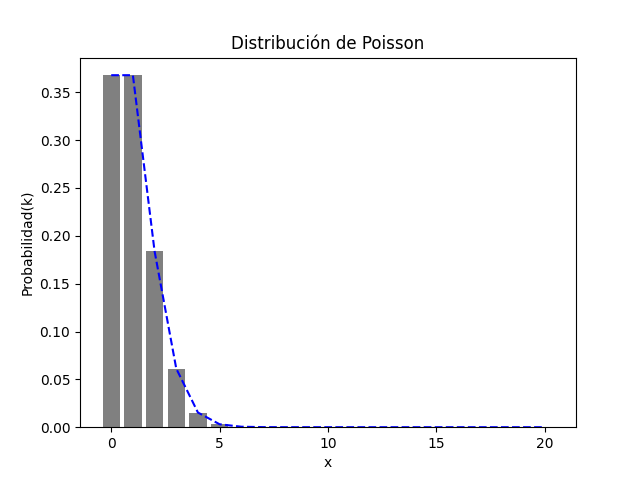
\includegraphics[scale=0.5]{figures/poisson_distribution_lambda_1.png}
  \end{center}
\end{frame}

\begin{frame}{Función de distribución de Poisson}
  \begin{block}{Ejemplo}
    El número de incidentes de tránsito que ocurren en una cierta avenida en un día
    cualquiera sigue una distribución Poisson de media $\lambda=4$. Entonces:
  \end{block}
  \begin{center}
    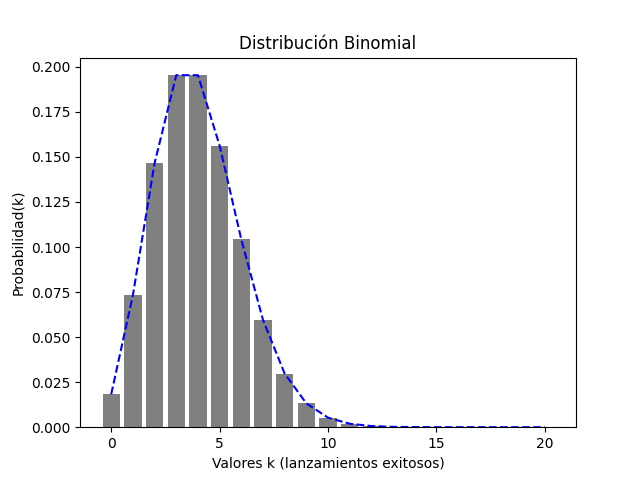
\includegraphics[scale=0.5]{figures/poisson_distribution_lambda_4.png}
  \end{center}
\end{frame}

\begin{frame}{Función de distribución de Poisson}
  \begin{block}{Ejemplo}
    El número de incidentes de tránsito que ocurren en una cierta avenida en un día
    cualquiera sigue una distribución Poisson de media $\lambda=10$. Entonces:
  \end{block}
  \begin{center}
    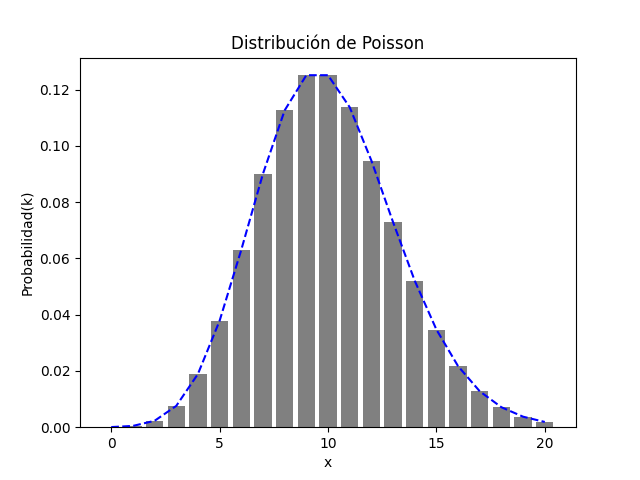
\includegraphics[scale=0.5]{figures/poisson_distribution_lambda_10.png}
  \end{center}
\end{frame}

\end{document}

